\begin{appendices}

\section{Worden's Strong Product}\label{secA1}

This is not the case for the next model product we define, as we will see this so-called “strong product" may have edges that are not present in the naive or modified products. The intent of adding these additional edges to the strong product is to allow certain state transitions to happen simultaneously where they could only happen separately in the naive or modified product. There are several potential ways to define a strong product, see Figures \ref{fig:strong_product_1}, \ref{fig:strong_product_2}, and \ref{fig:strong_product_3} for examples, but below we state the definition that we believe most closely aligns with that in \cite{worden2017products}.

\begin{definition}[Strong Product]
     Let $D^a = (V^a, E^a, F^a)$ and let $D^b = (V^b, E^b, F^b)$, let $D^a\Box D^b = D^c = (V, E^c, F^c)$. 
     
     Let $E^a_0$ and $E^b_0$ denote the edges of $D^a$ and $D^b$ that have flow rate functions with non-empty contagious sets. Then we define
     \begin{equation}
        E^d = \{((w, x), (y, z))\in V\times V\vert (w, y)\in E^a_0, (x,z)\in E^b_0\}
     \end{equation}
     Of course every edge $e\in E_d$ is associated with an edge $e_a\in E^a$ and $e_b\in E^b$, we define
     \begin{equation}
        F^d = \{ f_{e_a}\cdot f_{e_b} \vert e\in E^d, f_{e_a}\in F^a, f_{e_b}\in F^b  \}
     \end{equation}
     We define $E=E^c\cup E^d$, $F^3=F^{c}\cup F^{3,d}$, and $D^3=(V, E, F^3)$. Then
     \begin{equation}
        D^a\boxtimes D^b = D^3
     \end{equation} We call $\boxtimes$ \textbf{the strong product}.
\end{definition}


Consider the two SIR models presented in Figure \ref{fig:multistrain_sir}, call the blue strain model $G$ and the red strain model $H$. Figure \ref{fig:modified_multistrain_product} illustrates the modified product of $G$ and $H$ (i.e. $G\Box H$). Figures \ref{fig:strong_product_1}, \ref{fig:strong_product_2}, and \ref{fig:strong_product_3} correspond to alternative definitions of the strong product (i.e. $G\boxtimes H$). Notice firstly that all three have $G\Box H$ as a proper submodel. Secondly, Figure \ref{fig:strong_product_1} represents all contagious compartments contributing to the flow from $SS$ to $II$, where as Figure \ref{fig:strong_product_2} represents only the compartment contagious with both strains contributing to that flow. Figure \ref{fig:strong_product_3} represents what we might call the “strongest product" where every change in status with respect to both pathogens can happen simultaneously.


\begin{figure}
    \centering
    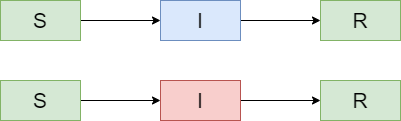
\includegraphics[width=\textwidth]{images/multistrain_SIR.png}
    \caption{Two SIR models representing unique strains of a pathogen}
    \label{fig:multistrain_sir}
\end{figure}

\begin{figure}
    \centering
    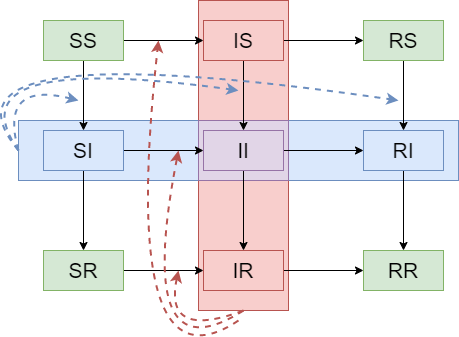
\includegraphics[width=\textwidth]{images/multistrain_modified_product.png}
    \caption{The modified product of the models given in Figure \ref{fig:multistrain_sir}}
    \label{fig:modified_multistrain_product}
\end{figure}

\begin{figure}
    \centering
    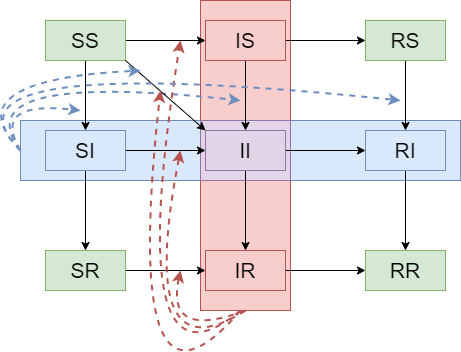
\includegraphics[width=\textwidth]{images/strong_product_type_1.png}
    \caption{One possible “strong product" of the models in Figure \ref{fig:multistrain_sir}}
    \label{fig:strong_product_1}
\end{figure}

\begin{figure}
    \centering
    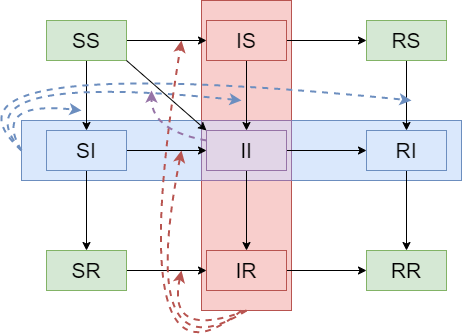
\includegraphics[width=\textwidth]{images/strong_product_type_2.png}
    \caption{One possible “strong product" of the models in Figure \ref{fig:multistrain_sir}}
    \label{fig:strong_product_2}
\end{figure}

\begin{figure}
    \centering
    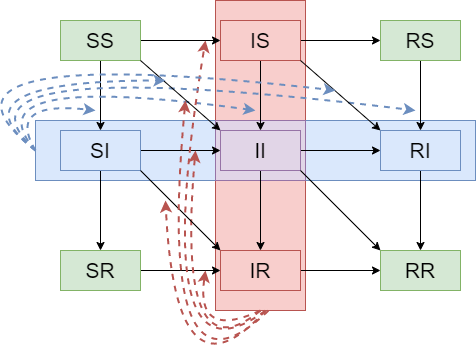
\includegraphics[width=\textwidth]{images/strong_product_type_3.png}
    \caption{One possible “strong product" of the models in Figure \ref{fig:multistrain_sir}}
    \label{fig:strong_product_3}
\end{figure}

\FloatBarrier

\section{Accumulator Compartments}\label{secB1}

Figure \ref{fig:vax_strat} depicts a possible stratification model with respect to vaccination status. Figure \ref{fig:vax_prod} depicts the product of the vaccination model with a simple SIR model. Sometimes modelers will want to keep track of the number of people that have changed status with respect to some aspect of the model, Figure \ref{fig:vax_acc} depicts this with relation to vaccination status. These so-called “accumulator compartments" cause difficulty for model products for two reasons. Firstly there is the fact that each unvaccinated compartment flows into the same accumulator compartment regardless of infection status, this could be overcome by splitting the total vaccination compartment into three separate compartments and summing them together after the fact. Secondly the outflow from each unvaccinated compartment is counted twice, once for the vaccinated compartment corresponding to the same infection status and once for the accumulator compartment. However we only want to subtract that outflow once from the source compartment.

\begin{figure}
    \centering
    
\includegraphics[width=\textwidth]{images/vax_strat.png}
    \caption{A vaccination stratification model}
    \label{fig:vax_strat}
\end{figure}

\begin{figure}
    \centering
    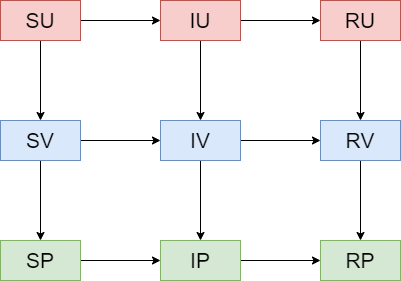
\includegraphics[width=\textwidth]{images/vax_prod.png}
    \caption{A vaccination stratified SIR model}
    \label{fig:vax_prod}
\end{figure}

\begin{figure}
    \centering
    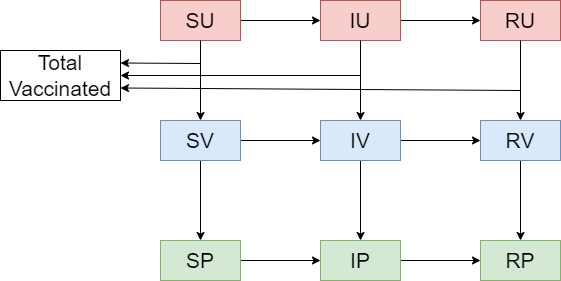
\includegraphics[width=\textwidth]{images/vax_accumulator.png}
    \caption{A vaccination stratified SIR model with an accumulator compartment}
    \label{fig:vax_acc}
\end{figure}

\FloatBarrier

\section{Age stratification in realistic examples}\label{secC1}

\subsection{Age Stratification}
    Let $G$ denote the epidemiological model depicted in Figure \ref{fig:macpan_base_epi}, $H$ denote the epidemiological model depicted in Figure \ref{fig:fh_base_epi}, and $T$ denote the age stratification model depicted in Figure \ref{fig:age_strat}. Then Figure \ref{fig:ageified_macpan_epi} depicts $G\Box T$ and Figure \ref{fig:ageified_fh_epi} depicts $H\Box T$.

\begin{figure}
    \centering
    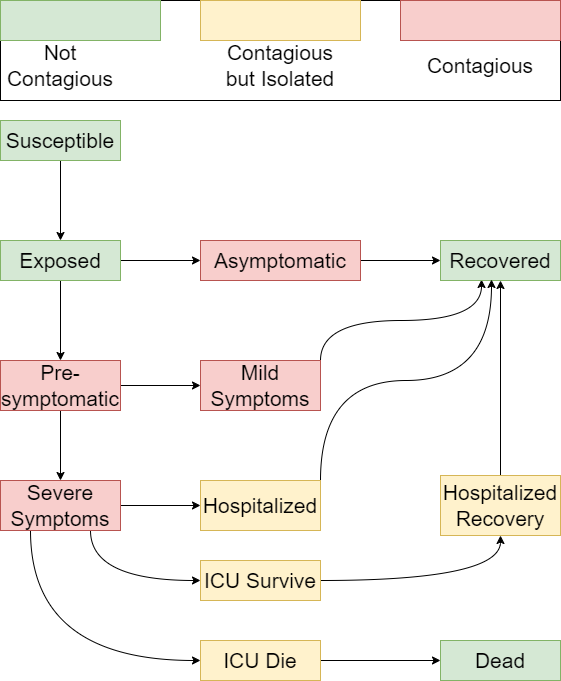
\includegraphics[width=\textwidth]{images/macpan_base_actual.png}
    \caption{The default epidemiological model used by macpan}
    \label{fig:macpan_base_epi}
\end{figure}

\begin{figure}
    \centering
    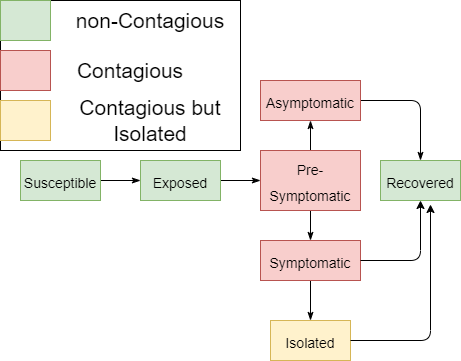
\includegraphics[width=\textwidth]{images/fieldshumphery.png}
    \caption{An alternate epidemiological model used by \cite{fields2021age}}
    \label{fig:fh_base_epi}
\end{figure}

\begin{figure}
    \centering
    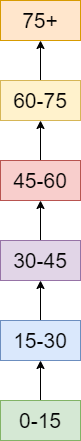
\includegraphics[width=0.25\textwidth]{images/age_stratification.png}
    \caption{An age stratification model}
    \label{fig:age_strat}
\end{figure}

\begin{figure}
    \centering
    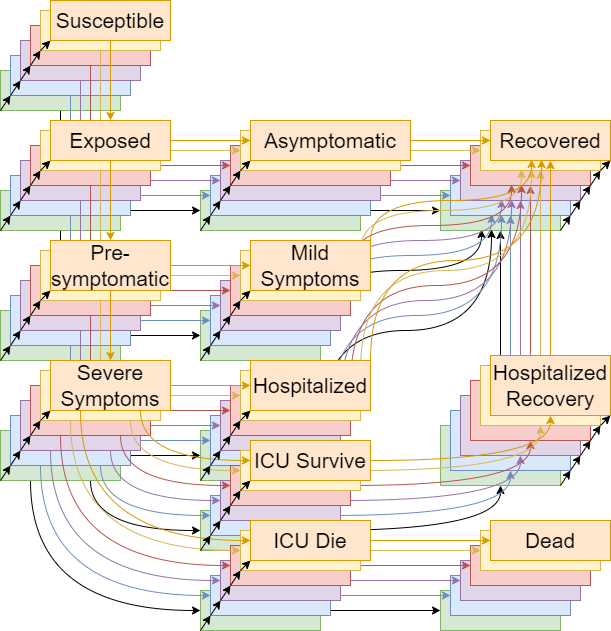
\includegraphics[width=\textwidth]{images/macpan_base_w_age.png}
    \caption{Macpan's base epi model age stratified}
    \label{fig:ageified_macpan_epi}
\end{figure}

\begin{figure}
    \centering
    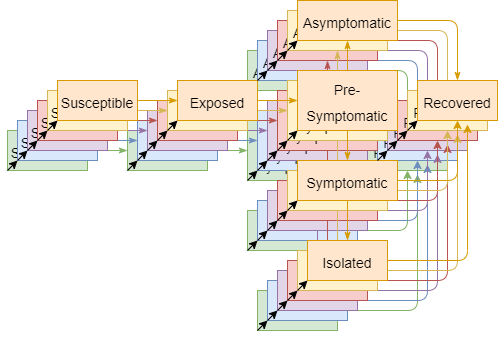
\includegraphics[width=\textwidth]{images/fieldshumphery_age.png}
    \caption{\cite{fields2021age} base epi model age stratified}
    \label{fig:ageified_fh_epi}
\end{figure}

\FloatBarrier

\end{appendices}
